A peephole optimiser rewrites assembly code to make ik more efficient, in terms of processor cycles or memory usage. The general procedure is (see figure~\ref{fig:diagram}):
\begin{enumerate}
\item assembly parsing;
\item division in basic blocks;
\item optimisation;
\item assembly generation.
\end{enumerate}
We discuss stages 1 and 4 first and then stage 2 and stage 3.

As an assembly program in the form of a set of text strings is difficult to process, the optimiser translates the input to an intermediate representation (ir) in the first stage. This translation is called \emph{parsing}. The resulting representation is a list of Python objects. After optimising, the resulting intermediate representation is translated back to assembly code. Ideally, when no optimisation is done between parsing assembly and regenerating assembly, the composite `function' $4\circ 1$ is the identity function on the set of all assembly programs. (In our implementation, only comments are left out in some cases, and spacing is sometimes changed.)

Stage 3

Stage 4



\begin{figure}[H]
\centering
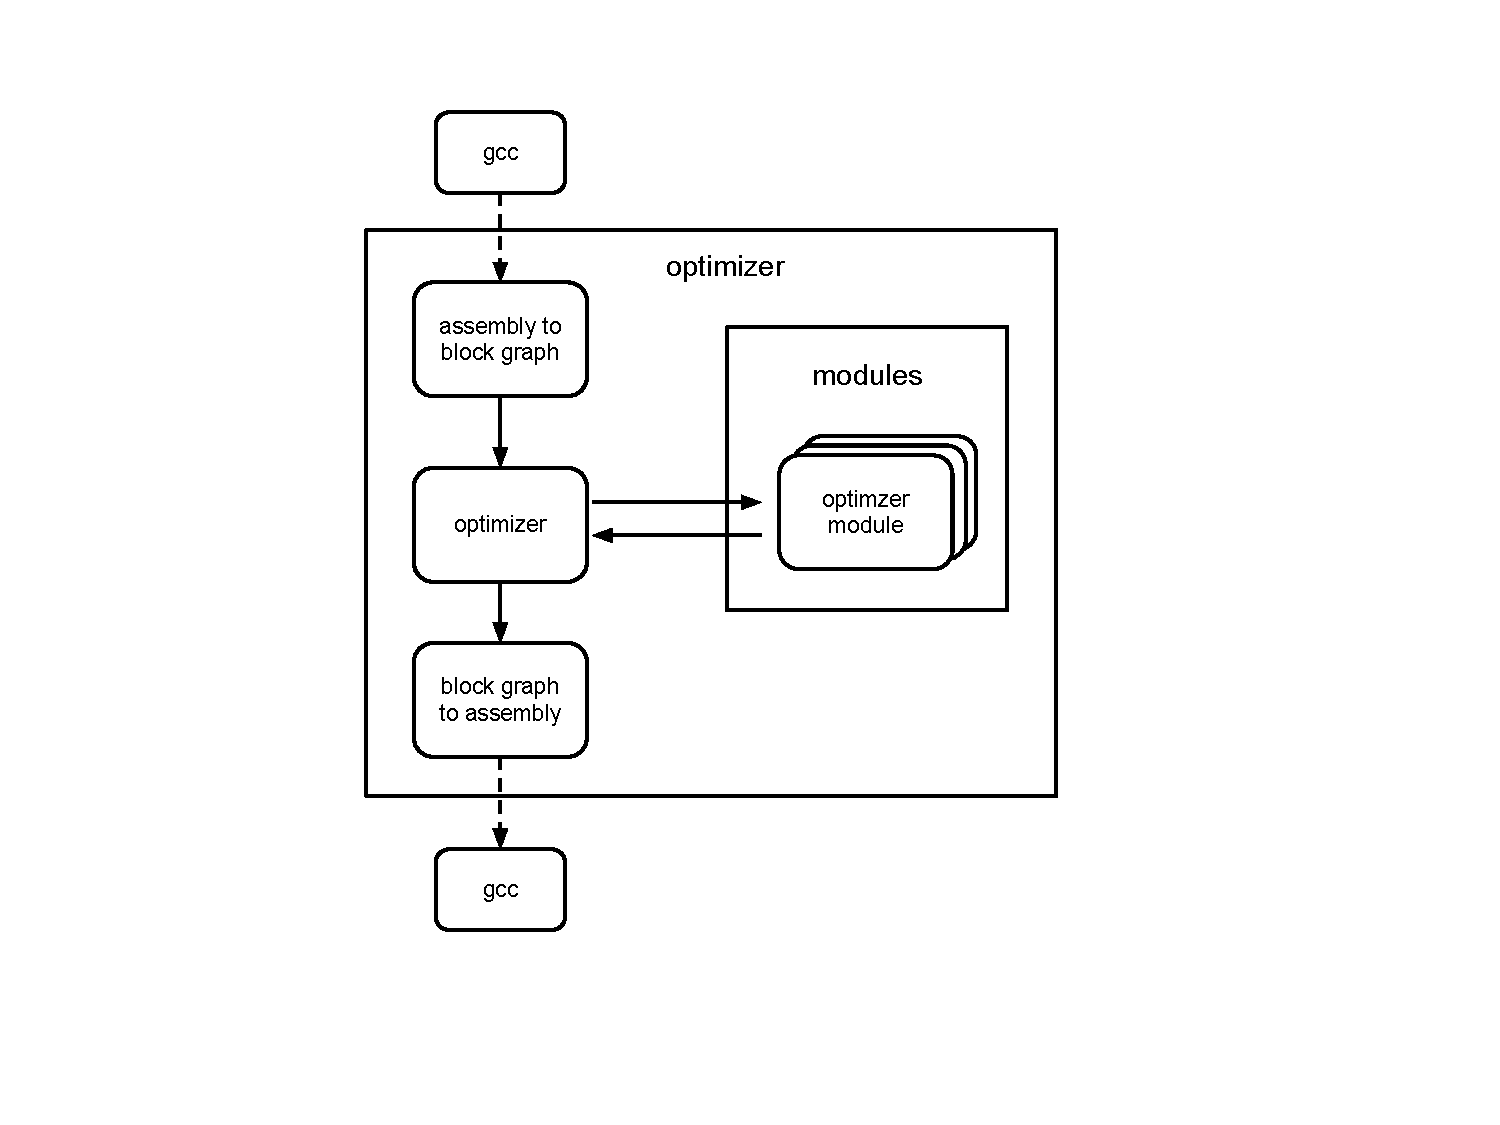
\includegraphics[viewport= 170 90 510 490, clip=true]{diagram}
\caption{Optimiser design diagram.}
\label{fig:diagram}
\end{figure}

